\lecture{6}{12. Februar 2025}{Mechanical Properties, Pt. 1: Elasticity}

\exercise{6.1}

\paragraph{(a)} Equations 6.4a and 6.4b are expressions for normal ($\sigma'$) and shear ($\tau'$) stresses, respectively, as a function of the applied tensile stress ($\sigma$) and the inclination angle of the plane on which these stresses are taken ($\theta$ of Figure 6.4). Make a plot showing the orientation parameters of these expressions (i.e., $\cos^2 \theta$ and $\sin \theta \cos \theta$) versus $\theta$.
\bigbreak
Equations 6.4a and 6.4b are respectively
\begin{align*}
  \sigma' &= \frac{F \cos\theta}{A_0 \cos\theta} = \sigma_0 \cos^2 \theta = \sigma_0 \left( \frac{1 + \cos 2 \theta}{2} \right) \\
  \tau' &= \frac{F \sin\theta}{A_0 / \cos\theta} = \sigma_0 \sin\theta \cos\theta = \sigma_0 \left( \frac{\sin 2\theta}{2} \right)
.\end{align*}
Therefore we will plot the following to expressions
\begin{gather*}
  \cos^2 \theta \\
  \sin\theta \cos\theta
.\end{gather*}
We get the following plot
\begin{figure} [ht]
  \centering
  \caption{Plot of $\cos^2 \theta$ and $\sin\theta \cos\theta$}
  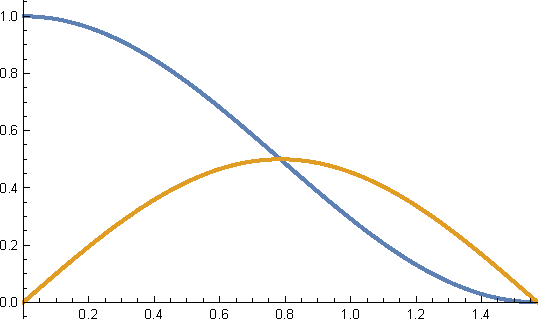
\includegraphics[width=0.5\textwidth]{plot_20250212_154046.pdf}
  \label{fig:e6_1}
\end{figure}
On \textbf{\autoref{fig:e6_1}} $\cos^2 \theta$ and $\sin\theta \cos\theta$ have been plotted. Their intersection is at $\frac{\pi}{4}$ and they both become 0 for $\frac{\pi}{2}$.

\paragraph{(b)} From this plot, at what angle of inclination is the normal stress a maximum?
\bigbreak
The normal stress has the orientation parameter $\cos^2 \theta$ (corresponding to the blue line) and it clearly has a maximum at 0. This also aligns with common intuition.

\paragraph{(c)} At what inclination angle is the shear stress a maximum?
\bigbreak
The shear stress has the orientation parameter $\cos\theta \sin\theta$ (corresponding to the red line) and it has a maximum at exactly $\frac{\pi}{4}$ also known as \qty{45}{\celsius}.


\exercise{6.2} A specimen of copper having a rectangular cross section $\qty{15,2}{mm} \times \qty{19,1}{mm}$ is pulled in tension with \qty{44500}{N} force, producing only elastic deformation. Calculate the resulting strain
\bigbreak
We know, from Hooke's law, that
\[ 
\sigma = E \epsilon
.\]
We can calculate the tensile stress $\sigma$ as
\[ 
\sigma = \frac{F}{A_0} = \frac{\qty{44500}{N}}{\qty{15,2}{mm} \cdot \qty{19,1}{mm}} = \qty{153,279}{MPa} 
.\]
The tension can then be calculated from Hooke's law, as we know $E_{copper} = \qty{130}{GPa}$ as
\[ 
\epsilon = \frac{\sigma}{E} = \frac{\qty{153,279}{MPa}}{\qty{130}{GPa}} = \num{1,18e-3} 
.\]



\exercise{6.5} A cylindrical rod of steel ($E = \qty{207}{GPa}$) having a yield strength of \qty{310}{MPa} is to be subjected to a load of \qty{11100}{N}. If the length of the rod is \qty{500}{mm}, what must be the diameter to allow an elongation of \qty{0,38}{mm}?
\bigbreak
The desired tension can be calculated as
\[ 
\epsilon = \frac{d}{l_0} = \frac{\qty{0,38}{mm}}{\qty{500}{mm}} = \num{7,6e-4}  
.\]
From the formula for stress $\sigma$ we can solve for the original area $A_0$ as
\[ 
\sigma = \frac{F}{A_0} \implies A_0 = \frac{F}{\sigma}
.\]
We also know that
\[ 
\sigma = E \epsilon
.\]
So the above becomes
\[ 
A_0 = \frac{F}{E\epsilon} = \frac{\qty{11100}{N}}{\qty{207}{GPa} \cdot \num{7,6e-4}} = \qty{70,557}{mm^2} 
.\]
From the formula for the area of a circle we can solve for $d$ as
\[ 
A = \pi \cdot r^2 = \pi \cdot \left( \frac{ø}{2} \right)^{2} \implies ø = \sqrt{\frac{4A}{\pi}}
.\]
We can substitute in the area of the rod to get
\[ 
ø = \sqrt{\frac{4A}{\pi}} \approx \qty{9,5}{mm} 
.\]
Therefore the steel rod should have a diameter of $ø = \qty{9,5}{mm}$.
